%%%%%%%%%%%%%%%%%%%%%%%%%%%%%%%%%%%%%%%%%
% Stylish Article
% LaTeX Template
% Version 2.1 (1/10/15)
%
% This template has been downloaded from:
% http://www.LaTeXTemplates.com
%
% Original author:
% Mathias Legrand (legrand.mathias@gmail.com) 
% With extensive modifications by:
% Vel (vel@latextemplates.com)
%
% License:
% CC BY-NC-SA 3.0 (http://creativecommons.org/licenses/by-nc-sa/3.0/)
%
%%%%%%%%%%%%%%%%%%%%%%%%%%%%%%%%%%%%%%%%%

%----------------------------------------------------------------------------------------
%	PACKAGES AND OTHER DOCUMENT CONFIGURATIONS
%----------------------------------------------------------------------------------------

\documentclass[fleqn,10pt]{SelfArx} % Document font size and equations flushed left

\usepackage[english, italian]{babel} % Specify a different language here - english by default

\usepackage{lipsum} % Required to insert dummy text. To be removed otherwise

\usepackage[defaultfam,light,tabular,lining]{montserrat} %% Option 'defaultfam'
%% only if the base font of the document is to be sans serig
\usepackage[T1]{fontenc}
\renewcommand*\oldstylenums[1]{{\fontfamily{Montserrat-TOsF}\selectfont #1}}
\renewcommand{\floatpagefraction}{.8} % for text coexisting with figs and tabs

\graphicspath{ {./images/} }

%----------------------------------------------------------------------------------------
%	COLUMNS
%----------------------------------------------------------------------------------------

\setlength{\columnsep}{0.55cm} % Distance between the two columns of text
\setlength{\fboxrule}{0.75pt} % Width of the border around the abstract

%----------------------------------------------------------------------------------------
%	COLORS
%----------------------------------------------------------------------------------------

\definecolor{color1}{RGB}{102, 102, 102} % Color of the article title and sections
%\definecolor{color1}{RGB}{178,34,34} % Color of the article title and sections
%\definecolor{color1}{RGB}{246,64,96} % Color of the article title and sections

%\definecolor{color2}{RGB}{0,20,20} % Color of the boxes behind the abstract and headings
%\definecolor{color2}{RGB}{246,64,96}

\definecolor{color2}{HTML}{a3b34f}

%----------------------------------------------------------------------------------------
%	HYPERLINKS
%----------------------------------------------------------------------------------------

\usepackage{hyperref} % Required for hyperlinks
\hypersetup{hidelinks,colorlinks,breaklinks=true,urlcolor=color2,citecolor=color1,linkcolor=color1,bookmarksopen=false,pdftitle={Title},pdfauthor={Author}}

%----------------------------------------------------------------------------------------
%	ARTICLE INFORMATION
%----------------------------------------------------------------------------------------

\JournalInfo{
\includegraphics[scale=0.35, trim = 0 6.7cm 1cm 3cm]{logo}}  
%Journal information
\Archive{ } % Additional notes (e.g. copyright, DOI, review/research article)

\PaperTitle{ArMeetup: \\
Explore the Meetup Social Network in ArangoDB} % Article title

\Authors{Dario Bertazioli\textsuperscript{1}, Fabrizio D'Intinosante\textsuperscript{1}, Massimiliano Perletti\textsuperscript{1}*} % Authors
\affiliation{\textsuperscript{1}\textit{Data Science, Department of Computer Science, University of Milano Bicocca, Milan, Italy}} % Author affiliation
\affiliation{*\textbf{Corresponding author}: m.perletti2@campus.unimib.it} % Corresponding author

\Keywords{AQL --- ArangoDB --- Cypher --- DataManagement --- DataVisualization --- Kafka --- Meetup --- Neo4j --- Nifi --- Python --- R --- SocialNetwork} % Keywords - if you don't want any simply remove all the text between the curly brackets
\newcommand{\keywordname}{Keywords} % Defines the keywords heading name

%----------------------------------------------------------------------------------------
%	ABSTRACT
%----------------------------------------------------------------------------------------

\Abstract{Meetup è una piattaforma che nasce con lo scopo di mettere in contatto le persone nella vita reale. 
Dopo la registrazione un utente può selezionare i propri interessi, iscriversi a gruppi locali e partecipare ad eventi. 
In questo elaborato si cerca di rispondere a diverse domande di ricerca tra le quali verificare, sfruttando misure qualitative, quale sia il giorno migliore della settimana e l'orario giornaliero più consono in cui organizzare un evento che riscuota successo, individuare l'area geografica approssimativa all'interno della quale un evento attrae utenti della piattaforma, o cercare di valutare l'efficacia del sistema di raccomandazione dell'applicazione. Questo lavoro è stato possibile grazie ai dati condivisi da Meetup tramite streaming RSVP. Da un punto di vista hardware è stata utilizzata la Virtual Machine Azure di Microsoft messa a disposizione dall'Università, mentre a livello di pipeline è stato sfruttato il software Nifi per effettuare lo streaming dei messaggi RSVP, Kafka per lo storage temporaneo e ArangoDB come database finale distribuito per poter effettuare le interrogazioni necessarie a rispondere alle domande di ricerca, permettendo inoltre di gestire in modo funzionale il grande volume di dati acquisito, con la possibilità di poter ulteriormente incrementarne il quantitativo grazie alla forte scalabilità orizzontale garantita dal database.}

%----------------------------------------------------------------------------------------

\begin{document}

\flushbottom % Makes all text pages the same height

\maketitle % Print the title and abstract box

\tableofcontents % Print the contents section

\thispagestyle{empty} % Removes page numbering from the first page

%----------------------------------------------------------------------------------------
%	ARTICLE CONTENTS
%----------------------------------------------------------------------------------------

\section*{Introduzione}
{\small %small for text larger
\textbf{Meetup} è una piattaforma creata nel 2002 con lo scopo di mettere in contatto le persone nella vita reale.\\
Una volta completata la fase di registrazione, gli utenti possono: \\
\\
- Selezionare i propri \textbf{interessi}: ciò avviene sottoscrivendo dei topic precompilati dall'applicazione in modo da favorire il sistema di raccomandazione. 
Questi topic spaziano tra i più svariati ambiti, da quello professionale a quello degli hobby, fino ai più comuni, relativi ad eventi sociali. \\
\\
- Iscriversi a \textbf{gruppi} locali: una volta selezionati i topic di interesse il sistema di raccomandazione dell'applicazione suggerisce all'utente una serie di gruppi più o meno locali (a seconda dell'area di interesse selezionata dall'utente) trattanti le tematiche in oggetto o altri argomenti ad essi correlati. 
Ciò permette agli utenti di incontrare persone della propria zona che condividono le stesse passioni. 
Nel caso in cui tra i topic di interesse per l'utente ce ne siano alcuni che non trovano nessun riscontro in gruppi presenti sul territorio, l'applicazione suggerisce all'utente di creare lui stesso un gruppo con oggetto quel topic, consigliando di mettersi in contatto con altre persone che dimostrano quell'interesse, suggerendole attraverso il sistema di raccomandazione.\\
\\
- Partecipare ad \textbf{eventi}: i gruppi locali, nel corso del tempo, organizzano eventi, incontri, meeting con oggetto i topic dichiarati dai gruppi stessi. 
Una volta che un gruppo ha organizzato un evento l'utente può visualizzarlo sulla propria home e, dopo aver visionato i dettagli, può decidere di comunicare la propria parteciperazione o la propria assenza e, nel caso volesse partecipare, può esplicitare l'intenzione di portare ospiti, il tutto in maniera non vincolante. 
Inoltre, per non restringere troppo la sfera di interessi degli utenti, l'applicazione permette anche di selezionare diversi filtri per la home, tra cui uno apposito per visualizzare eventi organizzati da gruppi di cui non si fa parte o un filtro ad hoc per visualizzare gruppi di cui l'utente non è già membro e che magari non trattano topic per cui l'utente ha dichiarato interesse, ma che essendo pur sempre gruppi locali, potrebbe gradire o trovare interessanti.\\
\\
Il focus centrale caratterizzante l'intero meccanismo dell'applicazione risulta quindi essere quello del "gruppo" visto come realtà associativa e fautore di momenti di aggregazione durante l'intero anno, molto spesso non guidati da una ristretta cerchia di organizzatori ma, al contrario, promotore di iniziative da parte dei propri membri. 
La varietà di gruppi spazia, a seconda dei topic trattati, tra:
\begin{enumerate}
\item Gruppi di socializzazione, che hanno come obiettivo principale quello di svolgere attività ludiche in compagnia, molto spesso anche promotori di veri e propri eventi di incontro per single;
\item Gruppi professionali, che si pongono l'obiettivo di mettere in contatto persone e professionisti di svariati campi attraverso workshop o presentazioni con il fine di fare crescere gli utenti dal punto di vista professionale;
\item Gruppi creativi, ovvero gruppi di progettazione e più vocati ad hobby ed alla pratica delle più svariate arti; \\
\end{enumerate}
Sintetizzando, quindi, la missione di Meetup è aiutare le persone a crescere e raggiungere i loro obiettivi attraverso connessioni autentiche e reali. \\
Ad oggi, Meetup è disponibile in 186 Paesi, e conta più di 40 milioni di membri sulla piattaforma, con più di 320 mila gruppi attivi ed una media di 12 mila eventi al giorno.
}
%------------------------------------------------

\section{Obiettivi}
{\small
Con l'analisi della rete sociale di Meetup e andando a studiare le relazioni che interconnettono le persone attraverso eventi sociali organizzati dai diversi gruppi presenti in tutto il globo è possibile ottenere una mappatura piuttosto dettagliata degli interessi comuni che portano ad agglomerare un significativo numero di soggetti instaurando relazioni tra di essi.
\\
\\
Cercando di indagare le caratteristiche di questa rete, pur tenendo in considerazione alcuni limiti (perlopiù temporali) dovuti all'acquisizione dati, ovvero quella avvenuta in forma streaming, i principali obbiettivi sono:
\begin{itemize}
\item Effettuare misure quantitative semplici per verificare in quali \textbf{paesi} la piattaforma è più utilizzata ed affermata;
\item Sfruttando le informazioni temporali, verificare quale sia il \textbf{momento migliore} della settimana e della giornata in cui organizzare un meetup per poter attrarre più persone possibili, considerando che la piattaforma è tipicamente utilizzata per incontri di carattere tecnico-professionale;
\item Servendosi di alcune informazioni spaziali, cercare di individuare quanto ampio sia il \textbf{raggio di un evento} in termini di attrazione degli utenti (ovvero, a che misura di distanza si trovano i membri che percorrono più strada per recarsi agli eventi ai quali partecipano);
\item Stimare l'\textbf{efficacia del sistema di raccomandazione} della piattaforma facendo uso combinato sia delle informazioni relative ai topic caratterizzanti gli eventi, sia di quelle relative a topic verso i quali gli utenti manifestano interesse al momento dell'iscrizione alla piattaforma, avendo sempre ben presente i limiti naturali imposti dalla durata finita e relativamente breve del periodo di streaming.
\end{itemize}
L'obiettivo del progetto, in sintesi, è quello di identificare correlazioni o tracce significative che possano determinare delle buone regole nella creazione di eventi di notevole impatto sociale; una piccola guida "\textbf{How to}" che illustri come debba  essere organizzato un meetup di successo.
}
%------------------------------------------------
\section{Implementazione: architettura}
{\small %FIXME: IMPORTANT: da aggiungere caratteristiche quali tolerance failure et similia un po' ovunque
\subsection{Temi trattati}
L'intera infrastruttura del progetto si pone come obiettivi didattici, oltre a quelli pratici già esposti, di affrontare due delle tre \textbf{V} caratteristiche dei \textit{Big Data}:
\begin{enumerate}
\item \textbf{V}elocity: attraverso l'applicazione di raccolta dei dati provenienti da una fonte streaming, con tutte le problematiche a questa connessa, come stabilità e durata della connessione e immagazzinamento dei dati in real time.
\item \textbf{V}olume: la raccolta dei dati ha prodotto un quantitativo di notevole importanza, comportando la costruzione di un DB di dimensione superiore ai 2 GB. Ciò ha comportato la necessità di applicare tecniche e tool adeguati a compiere task su grandi moli di dati in tempi accettabili.
\end{enumerate}
\subsection{Data source}%WebSocket (RSVP) Rest API
Meetup, come già detto, mette a disposizione parte dei dati in suo possesso relativi a membri iscritti alla piattaforma, gruppi creati ed eventi organizzati nella stessa. 
In particolare, i dati sono esposti in due modalità: 

\paragraph{streaming data:} 
la piattaforma condivide dati in streaming, composti essenzialmente da \textbf{RSVP}.
Le RSVP sono risposte di feedback da parte degli utenti che comunicano la propria partecipazione (o non partecipazione, in quanto le risposte possono essere anche negative), agli organizzatori di un evento.
Di seguito viene mostrato un esempio di struttura di un dato di questo genere (i messaggi sono nativamente in formato Json).%FIXME: add fig.
%da fare un format migliore
\newpage
\hrule
\vspace*{0.1cm}
Meetup RSVP:
\vspace*{0.05cm}
\hrule
\begin{itemize}[noitemsep]
\item \textbf{event}:
	\begin{itemize}[noitemsep]
	\item event\_id:	Unique alphanumeric identifier
	\item event\_name: Name of the event
	\item event\_url: URL to the full event page
	\item time: Event time if set in milliseconds since the epoch
	\end{itemize}
\item \textbf{group}:
	\begin{itemize}[noitemsep]
    \item group\_city: Group's home city
    \item group\_country: two-letter code of group's home country
    \item group\_id: Numeric identifier of the group
    \item group\_lat: Latitude of group's approximate location
    \item group\_lon: Longitude of group's approximate location
    \item group\_name: Name of the group
    \item group\_state: two-letter code of group's home state, if in US or CA
    \item group\_topics: Topics associated with this group
			\begin{itemize}[noitemsep]
			\item topic\_name: Longer name
        	\item urlkey: Unique keyword
			\end{itemize}
    \item group\_urlname: Unique portion of group's URL, no slashes
	\end{itemize}
\item guests: Number of guests the member is bringing
\item \textbf{member}: Member who RSVP'd
	\begin{itemize}[noitemsep]
    \item member\_id: Unique numeric id
    \item member\_name: Full name given
    \item other\_services: e.g. {"twitter": {"identifier": "MeetupAPI"}}
    \item photo: Thumbnail URL for member photo if one exists
	\end{itemize}
\item \textbf{mtime}: Last modified time of this RSVP, in milliseconds since the epoch
\item response: "yes" or "no"
\item rsvp\_id: Unique numeric identifier
\item \textbf{venue}: Venue, if public
	\begin{itemize}[noitemsep]
    \item lat: Latitude of the venue
    \item lon: Longitude of the venue
    \item venue\_id: Unique numeric identifier
    \item venue\_name
	\end{itemize}    
\end{itemize}
\hrule
\vspace*{0.2cm}
Si è proceduto ad estrarre tali dati da websocket, sfruttando Nifi (vedasi prossimo paragrafo).
\paragraph{rest API:} Meetup permette anche un accesso piuttosto flessibile ad ulteriori informazioni, esponendo tramite rest API dati riguardo a membri, gruppi ed eventi in formato JSON\footnote{Si veda \url{https://secure.meetup.com/meetup_api} per una lista dei metodi disponibili.}.
Abbiamo sfruttato questa possibilità per arricchire i dati acquisiti in streaming. 
In particolare, si è proceduto all'\textbf{enrichment} delle informazioni sui membri, integrando per ciascun utente:
\begin{itemize}[noitemsep]
\item la localizzazione spaziale, ovvero le coordinate geografiche (lat/lon) dichiarate in fase di registrazione così che il sistema di raccomandazione dell'applicazione possa suggerire gruppi su base geografica.
\item i topic per cui l'utente ha dichiarato di avere interesse al momento dell'iscrizione alla piattaforma, anche in questo caso per permettere il buon funzionamento del sistema di raccomandazione.
\end{itemize}
L'integrazione è avvenuta tramite http(s) request (a \url{https://api.meetup.com/2/members}) via python script, chiedendo alla rest API di restituire informazioni in base all'ID dello specifico membro, iterando quindi su tutti gli utenti.
Per ovviare al numero, piuttosto limitato, di richieste al minuto si è deciso di implementare un sistema a più chiavi, facendo un tuning della frequenza di richiesta in modo tale che risultasse appena al di sotto della soglia massima tollerata\footnote{Al di sopra della quale il client viene prima temporaneamente sospeso e poi bannato per ragioni di sicurezza e performance del servizio}.
Dunque, dopo aver partizionato in modo opportuno la lista di utenti in nostro possesso, si è proceduto all'enrichment con richieste parallele. 
Inoltre, si è preventivamente stimato il tempo totale necessario all'enrichment per tutti i (più di $800k$) membri con tre richieste parallele, controllando che fosse tollerabile.
\subsection{Nifi}% Producer and blabla
\begin{figure}
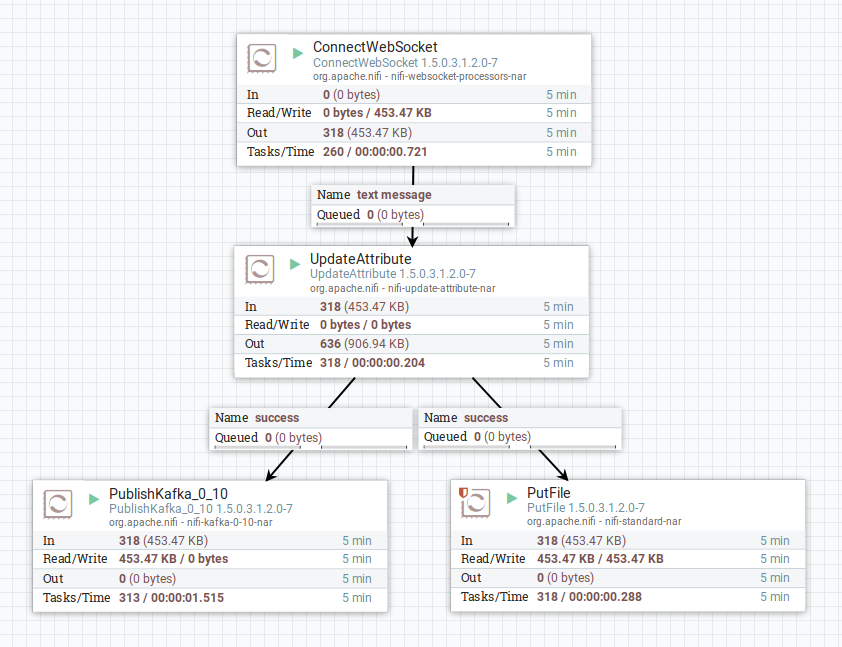
\includegraphics[scale=0.3]{images/nifi_workflow.png}
\caption{\footnotesize \label{nifi_workflow} Il workflow Nifi}
\end{figure}
Per acquisire i dati in streaming dalla piattaforma si è implementato un workflow di Nifi (vedasi \textbf{fig.~\ref{nifi_workflow}} \footnote{A clearer image:\url{https://gitlab.com/DBertazioli/armeetup/raw/master/report/images/nifi_workflow.png}}) contenente: 
\begin{itemize} %[noitemsep]
\item un nodo per la connessione alla \textbf{WebSocket} (\url{ws://stream.meetup.com/2/rsvps}), tramite un Client Jetty. 
\item un nodo per il parsing iniziale;
\item un nodo \textbf{PutFile}: si è deciso di salvare i dati acquisiti su file system per due motivi principali: innanzitutto ciò è utile per avere una copia di backup dei dati, qual ora si verificassero problemi (ad esempio, con il corretto setting di \textit{retention time} di Kafka); in secondo luogo, terminato il periodo di acquisizione, per facilitare la copia dei dati su altre virtual machines, in modo da implementare contemporaneamente la stessa pipeline su più macchine, per poter confrontare (quantitativamente, in termini, ad esempio, di quantità di dati importati, tempi di esecuzione dei vari scripts etc.) i risultati ottenuti;
\item un nodo \textbf{PublishKafka}, comodo per effettuare l'ingestion dei dati in Kafka, configurandosi come un vero e proprio producer. %FIXME: forse parentesi non necessaria
\end{itemize} 
I principali vantaggi che Nifi ha fornito sono: la gestione facilitata della queue, la possibilità di parsing online dei messaggi (i.e. tramite nodo UpdateAttribute, oppure RouteOnAttribute, per eventuali workflow più articolati) e la facile interfaccia con il Kafka Producer.
\subsection{Kafka}
Considerata la natura dei dati a nostra disposizione, che si ricorda consistere in un flusso di messaggi in streaming (RSVP), si è deciso di fare un ingestion in Kafka, potendo successivamente esplorare, iterare, e preprocessare le informazioni tramite Python API.
Vengono inoltre modificati i parametri di RetentionTime, in modo tale che Kafka funga anche da primo storage temporaneo, in grado di salvare all'interno di un topic tutti i messaggi acquisiti in real time streaming, per poi poterli processare successivamente senza correre il rischio di perdere qualche informazione.
Come accennato, con l'API di Kafka per Python si è potuto configurare un consumer per processare i dati, interfacciandosi poi con lo \href{https://gitlab.com/DBertazioli/armeetup/blob/master/py_scripts/python-arango_from_kafka.py}{script} per effettuare ingestion in real time nel database prescelto, e creando diversi \href{https://gitlab.com/DBertazioli/armeetup/tree/master/csv/struttura}{csv} per facilitare e rendere più efficiente l'import (bulk) nel database finale.
\subsection{Neo4j}% Storing and querying
\begin{figure}
\centering
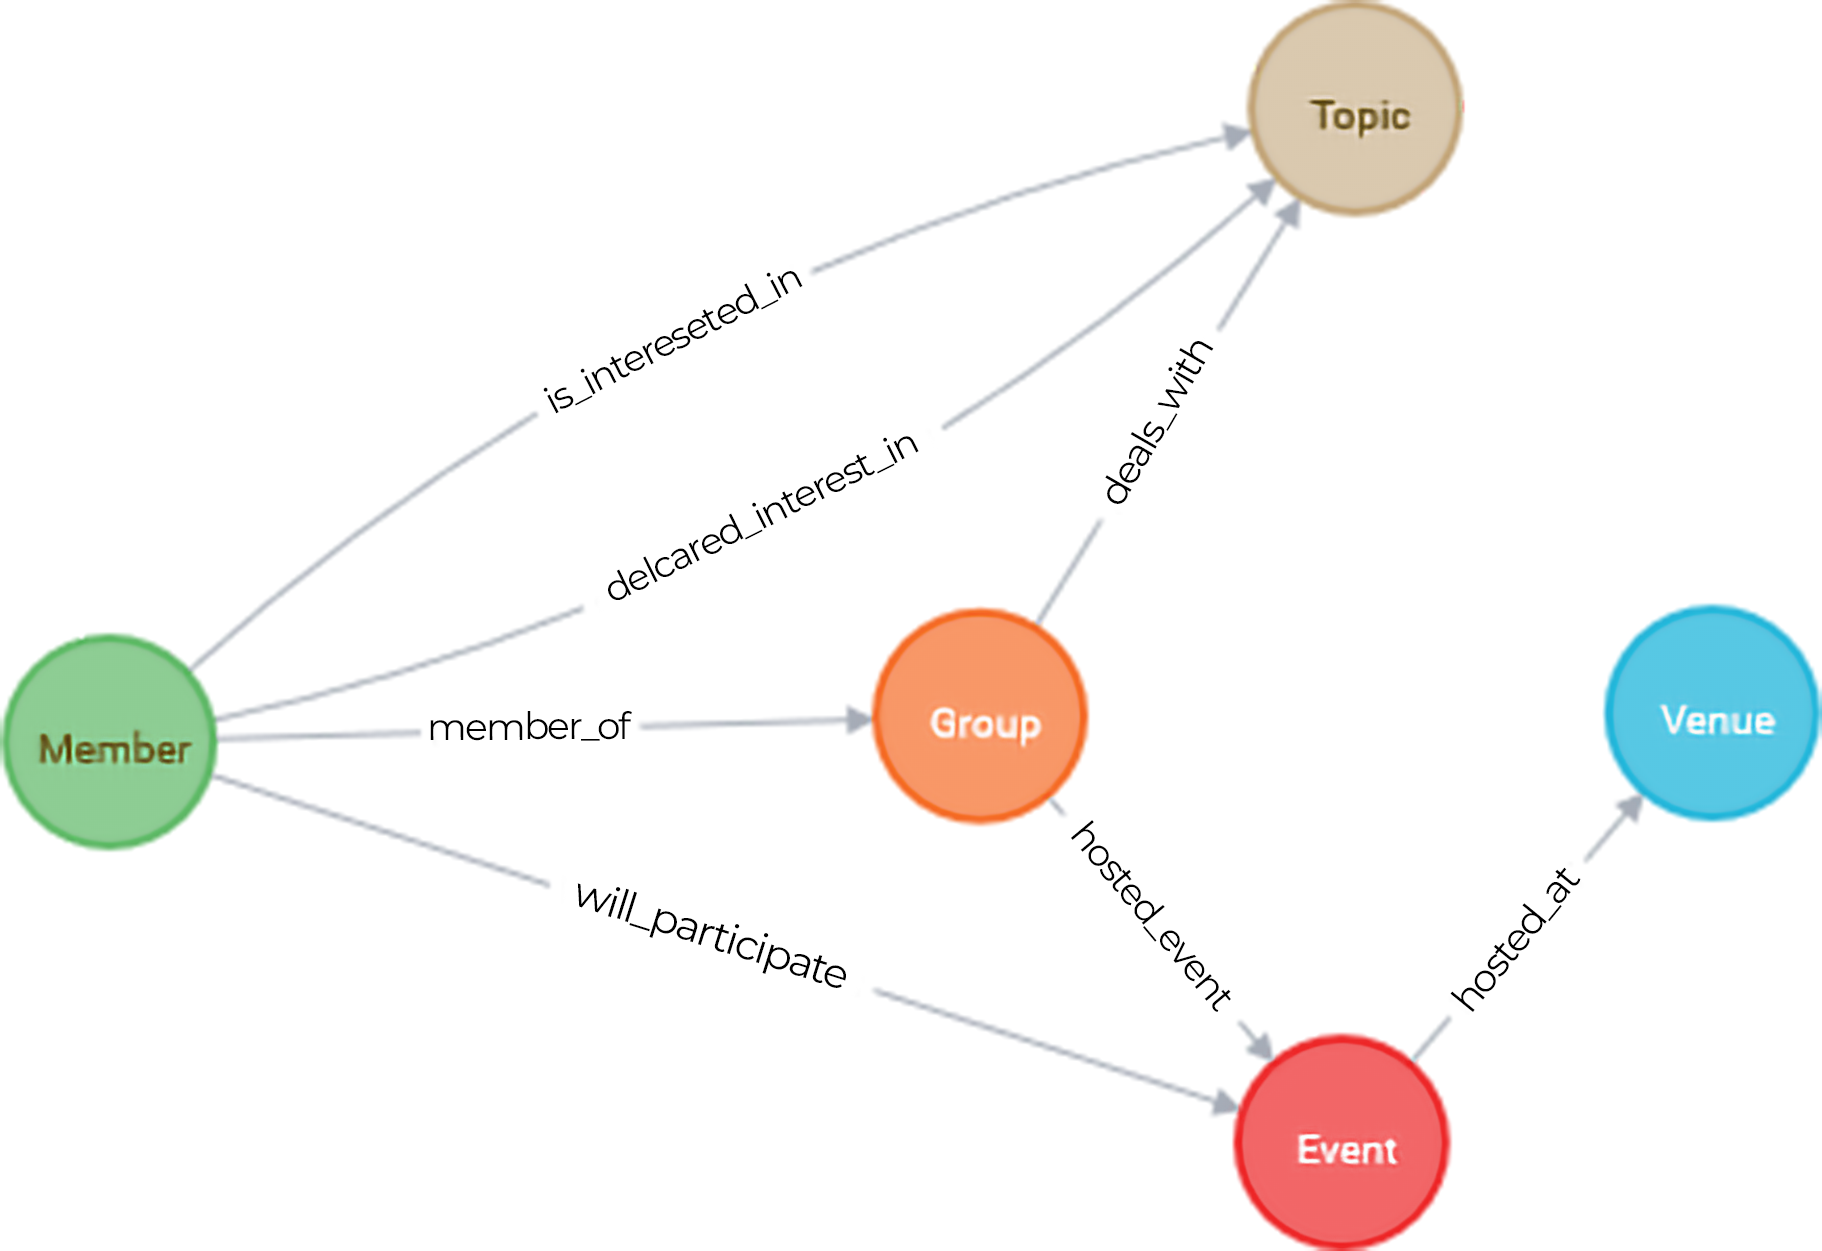
\includegraphics[scale=0.57]{graph.png}
\vspace*{0.01cm}
\caption{\footnotesize \label{graph_neo4j} Schema graph DB}
\end{figure}
Fin dal principio viene fatta la scelta di storare i dati in un database a grafo, per via della loro struttura naturale, che ben si presta ad essere schematizzata con nodi principali, proprietà e relazioni che interconnettono tali nodi. 
Viene quindi inizialmente effettuato l'import dei dati in Neo4j, sfruttando il linguaggio Cypher e l'ottimizzazione dell'import via csv, avendo inoltre sperimentato un approccio tramite l'API Python Py2Neo. 
Per facilitare un'eventuale serializzazione del processo di import, è stato creato uno script (Bash) che, una volta creati i csv, consente di automatizzare le varie chiamate alla cypher-shell, dato che il processo di creazione del database risulta piuttosto laborioso ma facilmente standardizzabile (\href{https://github.com/DBertazioli/NeoMeetup/blob/master/Scripts/import_cypher.sh}{import.sh}).
Questa soluzione però mal si prestava alla prospettiva di accumulare una grande mole di dati, anche in vista di un possibile ampliamento degli orizzonti del progetto, dato che Neo4j non permette la distribuzione orizzontale dei propri database ma giova soltanto di una scalabilità di tipo verticale. Per questo si è quindi deciso di avvalersi di un altro software.
\subsection{ArangoDB}
Data a questo punto l'esigenza di trovare una soluzione che coniugasse il bisogno di un database a grafo, ma che fosse anche in grado di essere scalabile orizzontalmente e quindi distribuibile in maniera trasparente all'utente (con processi e meccanismi interni al database) e non tramite segmentazione manuale dei dati all'origine, anche nell'ottica di voler eventualmente implementare uno streaming continuo dal RSVP API, si è optato per ArangoDB, un DBMS multi-modello in grado di unire i modelli documentale, a grafo e key-value, interrogabili con un unico e potente linguaggio di query condiviso (\texttt{AQL}, un misto tra un linguaggio \texttt{SQL-like} e un linguaggio di programmazione).
Sfruttando il particolare concetto di grafo implementato in ArangoDB è stata così realizzata una \textit{collection} per ogni vertice ed una \textit{edge-collection} per ogni arco del grafo. 
Nel caso di una ingestion di dati di notevole portata (e dimensione) la strategia di sharding da adottare, data la natura del software, può quindi basarsi sulla creazione di uno shard per ogni continente e specificare in fase di ingestion, per ogni collection e per ogni istanza il continente di riferimento \footnote{specificando in fase di creazione del database una strategia di sharding del tipo: \texttt{db.\_create("sharded\_collection", {"numberOfShards": 5, "shardKeys": ["continent"]})}}. 
Sulla base inoltre della disponibilità hardware è possibile creare più clusters, con conseguente possibilità di implementare una ulteriore strategia di frammentazione basata su specifici criteri.
Il database da noi creato, seguendo queste linee guida, presenta circa 1 milione e mezzo di singoli nodi e circa 28 milioni di relazioni tra questi, con un tempo di import su ArangoDB stimato in circa venti minuti.

\section{Risultati}
\paragraph{Misure quantitative semplici:}
con lo scopo di ispezionare attraverso alcune misure quantitative i dati in nostro
possesso, abbiamo interrogato il DB creato con alcune query per estrarre informazioni quali:
\begin{itemize}[noitemsep]
\item Quantità di eventi per Paese;
\item Quantità di gruppi per Paese;
\item Numero massimo di partecipanti agli eventi per Paese;
\item Numero medio degli ospiti portati da ogni partecipante agli eventi;
\item Trend topic per gli utenti;
\item Trend topic per i gruppi.
\end{itemize}
Come mostrato in \textbf{fig.~\ref{rose_plot}} i Paesi che presentano il più alto numero di gruppi attivi sono quelli anglofoni come USA e Gb, e sempre attraverso la visualizzazione sembrerebbe proprio che il numero totale di eventi organizzati in un Paese dipenda direttamente dal numero di gruppi attivi per quel Paese.
Anche per quanto riguarda il numero massimo di partecipanti agli eventi per Paese gli USA ovviamente spiccano per conformazione demografica rispetto ai paesi europei.
In merito invece ai trend topic, per i gruppi i più quotati sembrerebbero quelli inerenti benessere, argomenti sociali, divertimento ed impresa mentre, per gli utenti, i più presi in considerazione sembrerebbero quelli di tipo tecnologico ed inerenti la computer science.
\begin{figure}
\centering
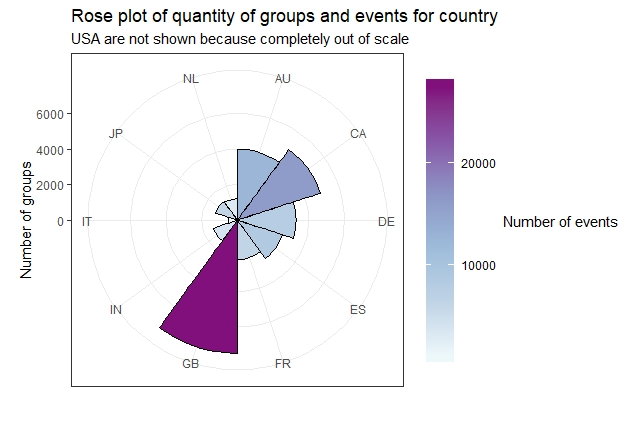
\includegraphics[width = 9.2 cm, height = 5 cm]{rose_plot_quantitative.jpeg}
\vspace*{0.01cm}
\caption{\footnotesize \label{rose_plot}Rose plot dei dieci paesi principali per
numero di gruppi ed eventi (gli USA, che sarebbero
di gran lunga i più rappresentati in tale plot, non
vengono inclusi perchè aventi numeri fuori scala)}
\end{figure}
\paragraph{Utilizzo delle informazioni temporali:}
attingendo alle informazioni temporali degli eventi, presenti nei messaggi, ed applicando un'opportuna manipolazione per convertire l'originale formato timestamp (time-from-epoch) in un formato umanamente più leggibile, si è stati in grado di rispondere alla seconda domanda di ricerca. 
Dopo aver infatti adattato i metadati temporali alle time zone così da avere una panoramica coerente sugli eventi Meetup tenutisi nel mondo, indipendentemente dal fuso orario, si è provveduto a realizzare una tabella di Pivot, tenente conto della numerosità di partecipanti agli eventi discriminati per giorno della settimana e per fascia oraria della giornata. 
Una volta realizzata la tabella è stato quindi possibile procedere alla costruzione della \textit{heatmap} in \textbf{fig.~\ref{plot_heatmap}} 
per rappresentare al meglio queste informazioni. 
Appare infatti chiaro dalla visualizzazione come i momenti migliori della settimana per organizzare un evento risultino essere il Martedì, il Mercoledì ed il Giovedì nella fascia oraria 18.00/20.00 ed il Sabato mattina tra le 10.00 e le 12.00. 
Ciò si conforma bene all'intuizione che la maggior parte dell'utenza di Meetup sembrerebbe essere rappresentata da lavoratori, professionisti, che sono quindi più propensi a partecipare ad eventi in orario successivo alla fine della giornata lavorativa o durante giorni non lavorativi, ma in questo caso prevalentemente la mattina.
\begin{figure}
\centering
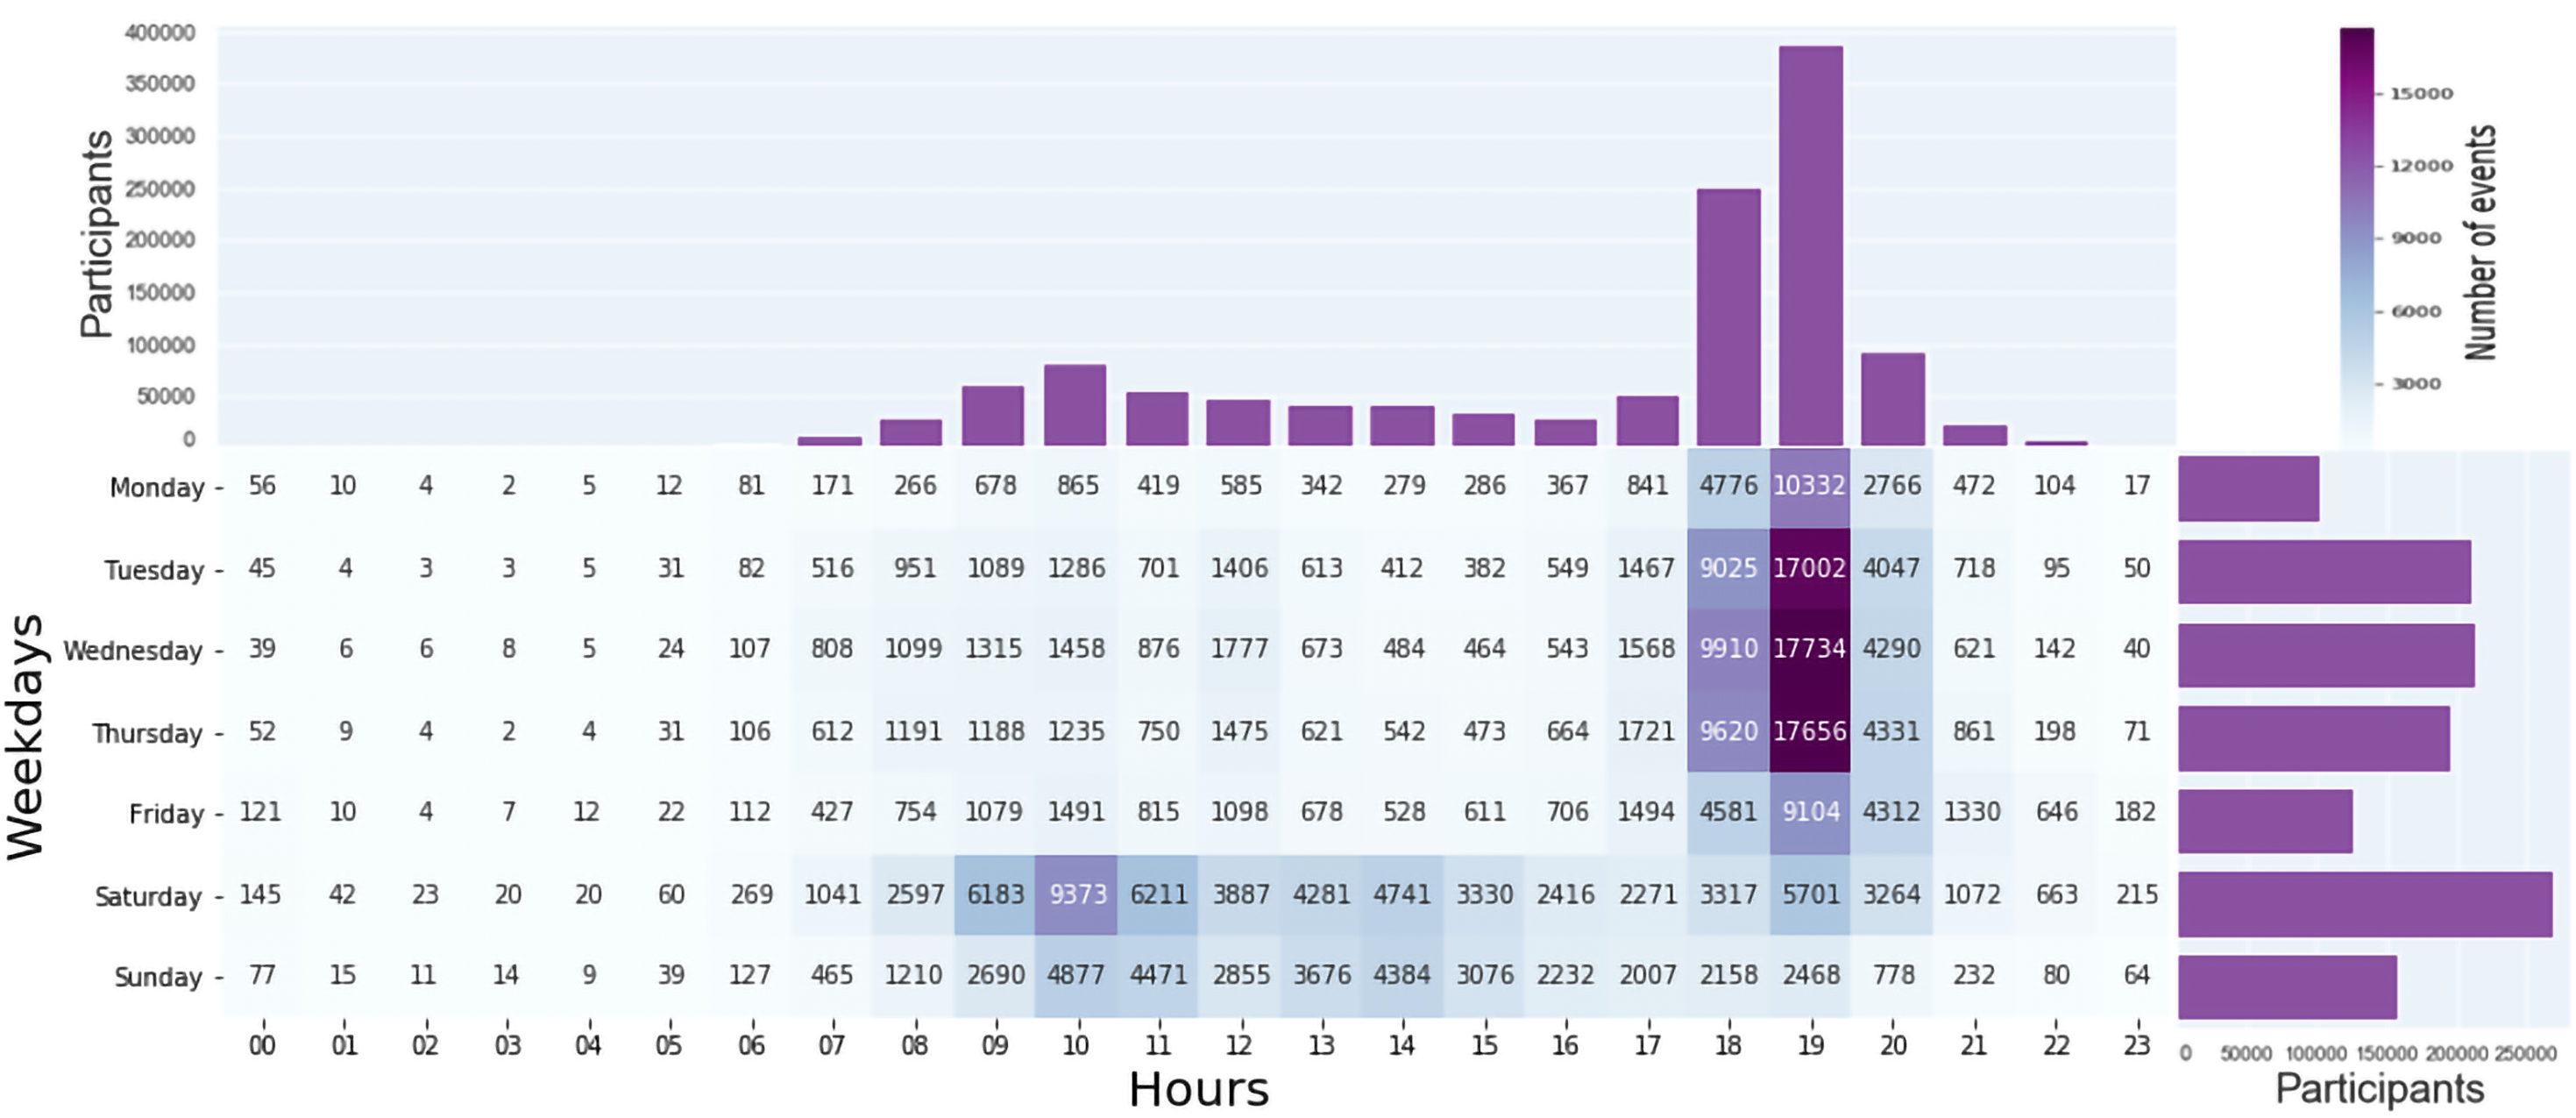
\includegraphics[width = 9.2 cm, height = 5 cm]{heatmap_with_barplot_v3.jpg}
\vspace*{0.01cm}
\caption{\footnotesize \label{plot_heatmap} Heatmap distribuzione temporale degli eventi}
\end{figure}
\paragraph{Utilizzo delle informazioni spaziali:}
per esplorare a fondo le informazioni a disposizione, si sono sfruttati i metadati spaziali presenti nei messaggi per realizzare una visualizzazione interattiva in formato di mappa esplorabile, focalizzata sull'Europa (principalmente per questioni di
potenza computazionale disponibile). 
Con questa mappa l'utente può potenzialmente esplorare l'offerta di eventi su base spaziale e visualizzarli localizzati nel luogo in cui sono stati organizzati e, cliccandoci sopra, può acquisire informazioni quali le caratteristiche dell'evento, come il nome dell'evento, il nome del luogo in cui è stato organizzato, l'orario, le keywords relative all'argomento trattato nell'evento e altro ancora. 
La mappa è stata costruita stratificando più layer, in modo da permettere all'utilizzatore di filtrare a priori ciò che potrà visualizzare, attraverso l'utilizzo di widget. 
Questi filtri permettono di focalizzare la visualizzazione su un certo Paese europeo, oppure di filtrare gli eventi sulla base dei topic trattati dagli stessi. 
Per limiti computazionali, inoltre, è stata effettuata una selezione a priori degli eventi, per cui sulla mappa saranno visibili solamente gli eventi che hanno raggiunto il più alto numero di adesioni, ma la struttura così come realizzata e in presenza di mezzi idonei potrebbe facilmente permettere di visualizzare la totalità degli eventi presenti a livello europeo o mondiale.
\paragraph{Valutazione efficacia sistema di raccomandazione:} $~~~$ con lo scopo di valutare il sistema di raccomandazione della piattaforma e sfruttando le informazioni a disposizione si è calcolata la Jaccard similarity per ogni utente, prendendo in considerazione i topic comuni tra quelli dichiarati dall'utente in fase di registrazione ed i topic dei gruppi di cui l'utente fa parte, come si vede in \textbf{fig.~\ref{jaccard_similarity}}. 
Questa misurazione ci ha permesso di giungere ad una certa constatazione riguardo la modalità di acquisizione dei dati. 
La misurazione risulterebbe viziata dalla raccolta dati tramite streaming poiché si è a conoscenza, per ogni utente, soltanto dei gruppi di cui fa parte condizionatamente al fatto che durante il periodo di streaming egli abbia risposto ad un evento organizzato da questi gruppi, e non della totalità dei gruppi a cui sarebbe iscritto. 
Questo particolare molto probabilmente contribuisce in maniera significativa alla determinazione di una bassa similarità tra i topic conformi ai gusti dichiarati dagli utenti e la totalità dei topic dichiarati sia dagli utenti che dai gruppi. 
Va inoltre tenuto conto che sia gli utenti in fase di registrazione che i gruppi al momento della creazione, molto probabilmente, prestano poca attenzione alla quantità e alla sparsità dei topic inseriti nel sistema, data anche la loro elevata granulosità, condizionando così la nostra misurazione. 
\begin{figure}
\centering
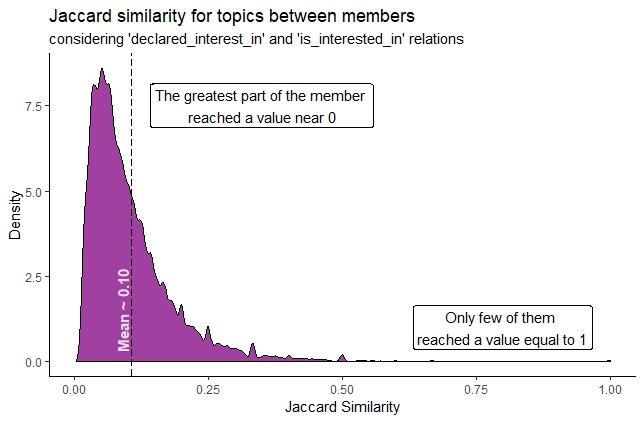
\includegraphics[width = 8.7 cm, height = 5 cm]{jaccard_similarity.jpeg}
\vspace*{0.01cm}
\caption{\footnotesize \label{jaccard_similarity} Jaccard similarity degli utenti riguardo i topic corrispondenti tra quelli dichiarati in fase di registrazione e quelli dei gruppi di cui fanno parte}
\end{figure}
%------------------------------------------------
\section{Sfide affrontate}

%FIXME: Ricordarsi di implementare un paragrafo che espliciti le caratteristiche tecniche del nostro sistema quali fault tolerance e cose varie (tutte le caratteristiche fornite da Nifi, Kafka e Arango basically)

{\small
Durante la realizzazione del progetto si sono dovute affrontare diverse problematiche legate ai più svariati ambiti, da quello della scalabilità in import dei dati a quello della velocità di processing, fino all'implementazione di una vera e propria costruzione continua del database con processo live streaming.
\paragraph{Symbolic Links:} avendo effettuato lo streaming utilizzando una sola Virtual Machine (VM), per poter trasferire i dati anche sulle altre macchine si è provveduto a creare parallelamente all'ingestion diretta in Kafka anche un backup direttamente nella macchina. 
Ciò ha permesso di trasferire direttamente questo backup dalla macchina principale alle altre. 
Successivamente nelle nuove VM si rendeva quindi necessario implementare un ingestion dalla VM a Kafka per mezzo di un workflow Nifi, così da emulare la stessa procedura dello streaming. 
Per ovviare poi ad un bug/limite dei nodi \textit{getFile/FetchFile} di Nifi, che si verifica nel tentativo di eseguire un ingestion di elevata quantità di file in una sola volta, è stata escogitata una soluzione creando dei link simbolici, dividendo la creazione in sottocartelle, facendo così leggere al nodo \textit{GetFile} questi link e impostando il nodo in modo che venisse eliminato il link dopo la singola lettura/ingestion. Ciò ha permesso di conservare i dati originali ed impedire che i nodi di import li eliminassero, facendo risparmiare tempo per quanto riguarda la creazione dei database di backup sulle diverse VM.
\paragraph{Ottimizzazione tempi di estrazione dei messaggi:}  $~~$ con il fine di estrarre le singole entità presenti nei messaggi, che per la natura dello streaming risultavano ripetersi più volte a seconda delle interazioni degli utenti con il servizio, si è tentato inizialmente un approccio mediante liste su python. 
Sinteticamente, questo approccio consisteva nel creare un Kafka consumer tramite l'API kafka per python e, ciclando, produrre tutti i messaggi in nostro possesso estraendo le singole entità, come utenti, gruppi e altro, utilizzando due liste di cui una contenitore per le singole entità ed una come "black list" per tenere traccia delle entità già inserite e quindi da non riprocessare. 
Questo approccio si è però dimostrato limitato in termini di perfomance nel processare grandi volumi di dati ed ha portato ad optare per una soluzione alternativa: utilizzando dei dizionari, e sfruttando gli ID presenti per ogni entità contenuta nei messaggi, si sono utilizzati questi ID come chiavi dei dizionari assegnandogli come valore tutte le proprietà associate a quell'entità. 
La differenza in termini di prestazioni si è dimostrata estremamente netta. 
Come si vede in \textbf{fig.~\ref{plot_lists_dicts}} la differenza è estremamente marcata, a partire dall'estrazione di più di 100 mila singole istanze il tempo richiesto dalle liste cresce esponenzialmente mentre quello dei dizionari resta sostanzialmente costante, per questo motivo per poter estrarre i CSV necessari all'import, su Neo4j prima e su ArangoDB dopo, si è deciso di adottare i dizionari.
\begin{figure}
\centering
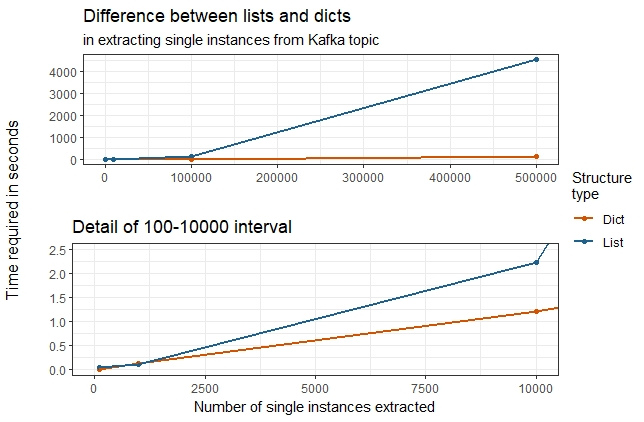
\includegraphics[scale=0.54]{viz_benchmark_lists_dicts.jpeg}
\caption{\footnotesize \label{plot_lists_dicts} Differenza di prestazioni fra liste e dizionari}
\end{figure}
\paragraph{Import Cypher vs Py2Neo:} una volta ottenuti i CSV necessari all'import dei nodi e delle relazioni si è innanzitutto tentato un approccio con l'API Py2Neo per python. 
Come per le liste in precedenza, l'API si è comportata bene sulle ridotte dimensioni, mentre al crescere del volume dei dati da importare si è resa inutilizzabile per gli elevati tempi d'attesa. 
Come si vede in \textbf{fig.~\ref{plot_cypher_py2neo}} l'import tramite cypher shell, meccanismo nativo di import per Neo4j, si dimostra fin dalle piccole dimensionalità molto più efficiente di Py2Neo mantenendo praticamente costante il tempo di import, con prestazioni che toccano circa i 12 secondi per importare 500 mila nodi distinti, contro i circa 80 minuti richiesti da Py2Neo.
\begin{figure}
\centering
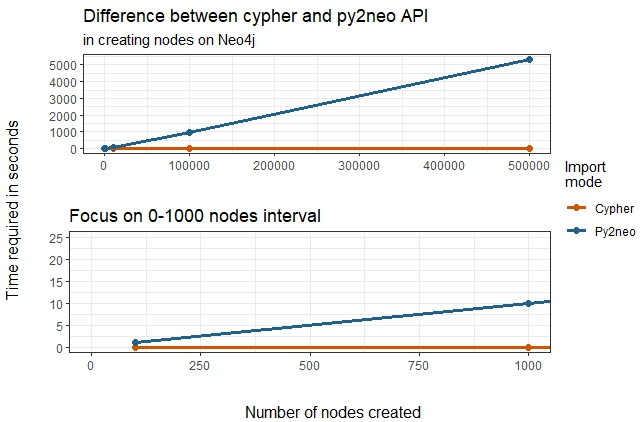
\includegraphics[scale=0.54]{viz_benchmark_cypher_py2neo.jpeg}
\vspace*{0.01cm}
\caption{\footnotesize \label{plot_cypher_py2neo} Differenza di prestazioni fra Cypher e Py2Neo API}
\end{figure}
\paragraph{Import Cypher vs Arangoimp:}
\begin{figure}
\centering
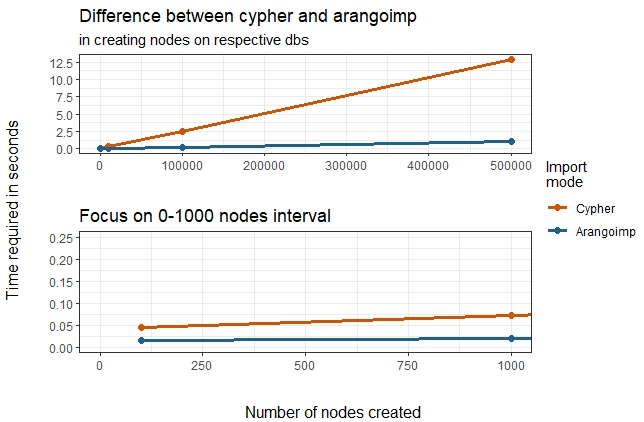
\includegraphics[scale=0.54]{viz_benchmark_cypher_arangoimp.jpeg}
\vspace*{0.01cm}
\caption{\footnotesize \label{plot_cypher_arangoimp} Differenza di prestazioni fra Cypher e Arangoimp}
\end{figure}
come si può vedere in \textbf{fig.~\ref{plot_cypher_arangoimp}} il confronto tra Cypher e Arangoimp nell'import dati si gioca sull'ordine dei millisecondi per piccole importazioni mentre di pochi secondi per grandi moli di dati. 
Arangoimp si dimostra sostanzialmente costante per i volumi testati, mentre l'import tramite Cypher comincia a crescere in termini di tempo richiesto partendo da volumi superiori a 100mila istanze. 
Anche per quanto riguarda l'import delle relazioni tra i nodi Arangoimp si è dimostrato molto più rapido. 
Questo probabilmente è ascrivibile al fatto che Neo4j sfrutta un meccanismo chiamato Index free adjacency che permette di incrementare le prestazioni a livello di query a discapito di una maggiore lentezza in fase di import. 
\paragraph{Scalability:} in prima istanza, dopo un primo streaming effettuato alla fine di dicembre 2018, si sono sfruttati questi dati per calibrare le scelte in fatto di gestione della dimensionalità. 
Questo primo streaming contava circa 1 milione di messaggi provenienti dall'API Meetup. 
Proprio grazie a questo quantitativo iniziale si sono potute tarare le nostre decisioni su una dimensionalità realistica e già piuttosto complessa. 
Per questa ragione si è deciso di sfruttare in prima istanza Kafka, che ha permesso di effettuare il primo storage senza essere condizionato in fase di consuming dalla dimensionalità dello storage stesso. 
Anche la scelta di un database a grafo, e nello specifico di Neo4j in principio, è stata presa con l'intento di ottenere il massimo delle prestazioni possibili in fatto di velocità di risposta alle query, anche se poi sostituito successivamente dall'adozione di ArangoDB, ancora più performante in fase di import, e con la possibilità di essere distribuito orizzontalmente. 
Infine le scelte operate in fatto di processing dei dati con i dizionari per l'estrazione delle singole entità prima, e con l'applicativo Arangoimp per l'import su ArangoDB dopo, si sono dimostrate essere vincenti per quello che è stato il vero e proprio streaming effettuato a febbraio 2019.
Quest'ultimo infatti contava più di 2 milioni e mezzo di messaggi, con una dimensionalità finale del database di 1 milione e mezzo di singoli nodi e circa 28 milioni di relazioni tra questi.
\paragraph{Conversione dei metadati temporali:} durante la fase di analisi dei dati con l'obiettivo di realizzare statistiche e visualizzazioni, ci si è imbattuti nel problema della formattazione dei metadati temporali. 
Nello specifico tutti i metadati temporali provenienti dall'API di Meetup si presentano in formato timestamp in millisecondi con fuso orario UTC; questo rappresentava un problema nella rappresentazione temporale degli eventi ad esempio, oppure per quella della sottoscrizione agli eventi da parte degli utenti. 
Per ovviare a questo inconveniente, e formattare questi metadati in formato date-time condizionati alle rispettive time-zone locali si sono sfruttati i metadati riguardanti la localizzazione degli utenti al momento della sottoscrizione agli eventi e, quindi, alla generazione del messaggio RSVP. 
Partendo quindi da queste informazioni in formato latitudine/longitudine si sono innanzitutto localizzate le corrispondenti time-zone attraverso la libreria \textit{timezonefinder} per python e, successivamente, attraverso la libreria \textit{pytz} si sono potuti convertire i timestamp in date-time condizionatamente alla time-zone prima definita. 
Lo sviluppo dei dati è visibile in \textbf{fig.~\ref{datetime_timezoned}}, dove è possibile visualizzare come il dataset si sia trasformato durante i passaggi descritti.
\begin{figure}
\centering
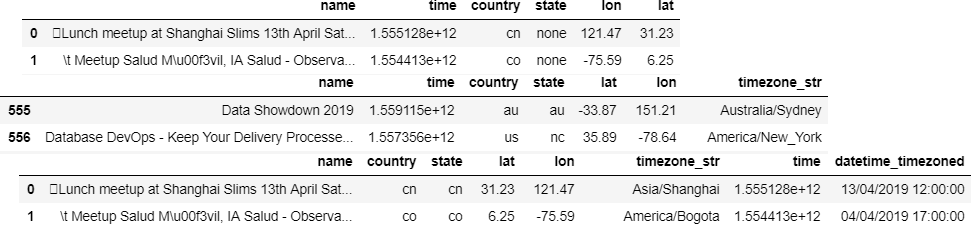
\includegraphics[width = 9 cm, height = 3.5 cm]{datetime_timezoned.PNG}
\vspace*{0.01cm}
\caption{\footnotesize \label{datetime_timezoned} Passaggi conversione timestamp into datetime timezoned}
\end{figure}
\paragraph{Implementazione ingestion database in live streaming:}
con l'obiettivo di implementare il meccanismo di ingestion continuo nel DB, sulla base di uno streaming no-stop, si è implementata una pipeline che, a partire dal consumer Kafka, acquisisce i messaggi, li elabora con lo stesso meccanismo utilizzato per creare i csv e, sfruttando \textit{python-arango}, un API di interfaccia tra python e ArangoDB, effettua l'ingestion nel database, preservandone la consistenza effettuando un check per evitare di inserire duplicati. 
Per questa fase di ingestion sono previste due possibili strategie:
\begin{itemize}[noitemsep]
\item Un ingestion continua, per cui ogni messaggio viene inserito nel DB in seguito al check della consistenza;
\item Una ingestion "a blocchi" di dimensione variabile a piacere, la quale consiste nel creare dei batch db tramite l’API, per cui si raccolgono un determinato
numero di messaggi e si effettua un caricamento più consistente\footnote{Ad esempio, c’è la possibilità di effettuare una ingestion al giorno, programmando nella Crontab unix l’esecuzione di un determinato script di import} .
\end{itemize}
Per testare la tenuta della pipeline si è effettuata l'ingestion di tutti i circa 2 milioni di messaggi precedentemente archiviati in Kafka, verificando quindi la resistenza ad un grande carico: tipicamente infatti la frequenza dei messaggi oscilla tra i 100 ed i 300 messaggi al secondo, ben al di sotto delle frequenze testate, ovvero tra 1000 e 10 mila messaggi al secondo.
}
\section{Conclusioni}
Grazie alla pipeline di acquisizione, trattamento, enrichment parziale e storage dei dati RSVP esposti da Meetup siamo stati in grado di rispondere alle domande di ricerca poste all'inizio di questo lavoro, definendo un quadro piuttosto generale che descrive le caratteristiche salienti (la struttura di meetup), i punti di forza (l'aggregazione e la partecipazione attiva degli utenti) e le statistiche in termini di diffusione, utilizzo e ricchezza della proposta di contenuti sulla piattaforma di tale organizzazione. 

Vale la pena di sottolineare che la struttura software da noi creata beneficia delle seguenti principali caratteristiche:
\begin{itemize}
\item Scalability: la scalabilità del DB è garantita dal DBMS scelto, siccome ArangoDB permette di scalare orizzontalmente in modo praticamente illimitato.
\item Fault tolerance: con la dovuta distribuzione e replicazione della pipeline su diverse macchine, sarebbe potenzialmente garantita la tolleranza all'interruzione di un qualsiasi elemento all'interno della pipeline stessa. Ciò sarebbe permesso in particolare da Nifi e Kafka che garantiscono la possibilità di gestire la queue.
\item Consistency: la consistenza è garantita dalla pipeline di preprocessing elaborata, in grado di garantire l'univocità delle istanze. Con un ulteriore raffinamento di quest'ultima sarebbe possibile inoltre correggere anche le piccole imperfezioni rimaste, come la riconversione di alcuni caratteri speciali nei testi.
\end{itemize}

Il compimento di questo progetto ci è stato particolarmente utile perchè ci ha permesso di fare pratica con una serie di software ampiamente diffusi in ambito di data management (Nifi, Kafka, Neo4j, ArangoDB e le varie API connesse). 

Inoltre, ci siamo dovuti scontrare con una serie di sfide e necessità pratiche che ci hanno fatto comprendere alcune delle principali difficoltà (come ad esempio il tuning della pipeline per avere performance accettabili, oppure le difficoltà con il (pre)processing dei dati grezzi e il loro parziale arricchimento) che tipicamente si incontrano qualora si voglia strutturare un progetto (anche, a maggior ragione, non di tipo "didattico") come quello in oggetto.
\section*{Ringraziamenti} % The \section*{} command stops section numbering
Per questo lavoro si ringraziano
\begin{itemize}
\item Il prof. Andrea Maurino per gli opportuni indirizi ed i consigli, oltre che per l'opportunità di cimentarci con un problema che ci ha fatto crescere professionalmente;
\item Il prof. Vincenzo Cutrona per la costante presenza e pazienza nei momenti di bisogno;
\item Il prof. Antonio Cabitza per tutti i consigli datici per rappresentare al meglio i risultati del nostro lavoro, in modo da valorizzarlo ancora di più;
\item Il nostro compagno, e amico, Alessandro Borroni, per aver realizzato per noi il logo del progetto;
\item L'Università degli Studi di Milano-Bicocca per averci fornito l'accesso alla macchine virtuali su Microsoft Azure, così da permetterci di lavorare all'interezza del nostro progetto.
\end{itemize}
\addcontentsline{toc}{section}{Ringraziamenti} % Adds this section to the table of contents

%So long and thanks for all the fish.

%----------------------------------------------------------------------------------------
%	REFERENCE LIST
%----------------------------------------------------------------------------------------
\phantomsection
\bibliographystyle{unsrt}
\bibliography{sample}

%----------------------------------------------------------------------------------------

\end{document}